\subsection{Trajectory Length}
%
%\subsection{Cloud Techniques: Elastic Search}
%
%What if we re-provision resources in response to events outside the
%application's control, such as a slow Lustre.
%
%\subsection{Future work}
%
%How Much: cache policy from past, regime detection, Belady's Min

\section{Cache Management Using System Architecture Knowledge}
\label{sec:arch-specific}

Using the Mantle policy engine, we test a variety of cache management tools and
algorithms on a single in-memory database node using the keyspace analysis in
Section~\S\ref{sec:parsplice-keyspace-analysis}. These strategies are
implemented as the ``when" and ``how much" policies from the Mantle API; the
``where" callback does not make sense for a single node (segments are either in
the cache or they are not). The evaluation metric is the accuracy and runtime
of each strategy; the strategy should be accurate enough so as to sacrifice
negligible performance and fast enough to run as often as we want to detect key
access patterns. The goal of the following sections is not to find an optimal
solution, as this can be done with parameter sweeps for thresholds; rather, we
try to find techniques that work for a range of inputs and system setups.

First we sized the cache according to our system specific knowledge. By
``system", we mean the hardware and software of the storage hierarchy. We look
at request rate, unique keys in a sliding window, and bandwidth capabilities. For
example, we know that LevelDB cannot handle high IO request rates.

% technical details
In the original ParSplice implementation, each cache node uses an unlimited
amount of memory to store segment coordinates. We limit the size of the cache
using an LRU eviction policy, where the penalty for a cache miss is retrieving
the data from the persistent database.  We evict keys (if necessary) at every
operation instead of when segments complete because the cache fills up too
quickly otherwise.

The results for different cache sizes for a growth rate of \(\Delta_1\) over a
2.5 hour run across 256 workers is shown in
Figure~\ref{fig:methodology-tradeoff}.  ``Baseline" is the performance of
unmodified ParSplice  measured in trajectory duration (\(y\) axis) and
utilization is measured with memory footprint of just the cache (\(y2\) axis).
The other graph shares the \(y\) axis and shows the trade-off of using a basic
LRU-style cache for different cache sizes, implemented using a ``when" policy
of \texttt{server[whoami]['cachesize']>n} and a ``how much" policy of
\texttt{servers[whoami]['cachesize']-n}. The error bars are the standard
deviation of 3 runs. 
%\begin{figure}[h] \footnotesize \begin{minted}{lua}
%server[whoami]['cachesize'] > n \end{minted} \end{figure}

%and ``how much":
%\begin{figure}[h]
%\footnotesize
%\begin{minted}{lua}
%servers[whoami]['cachesize'] - n
%\end{minted}
%\end{figure}


\begin{figure}[t]
\noindent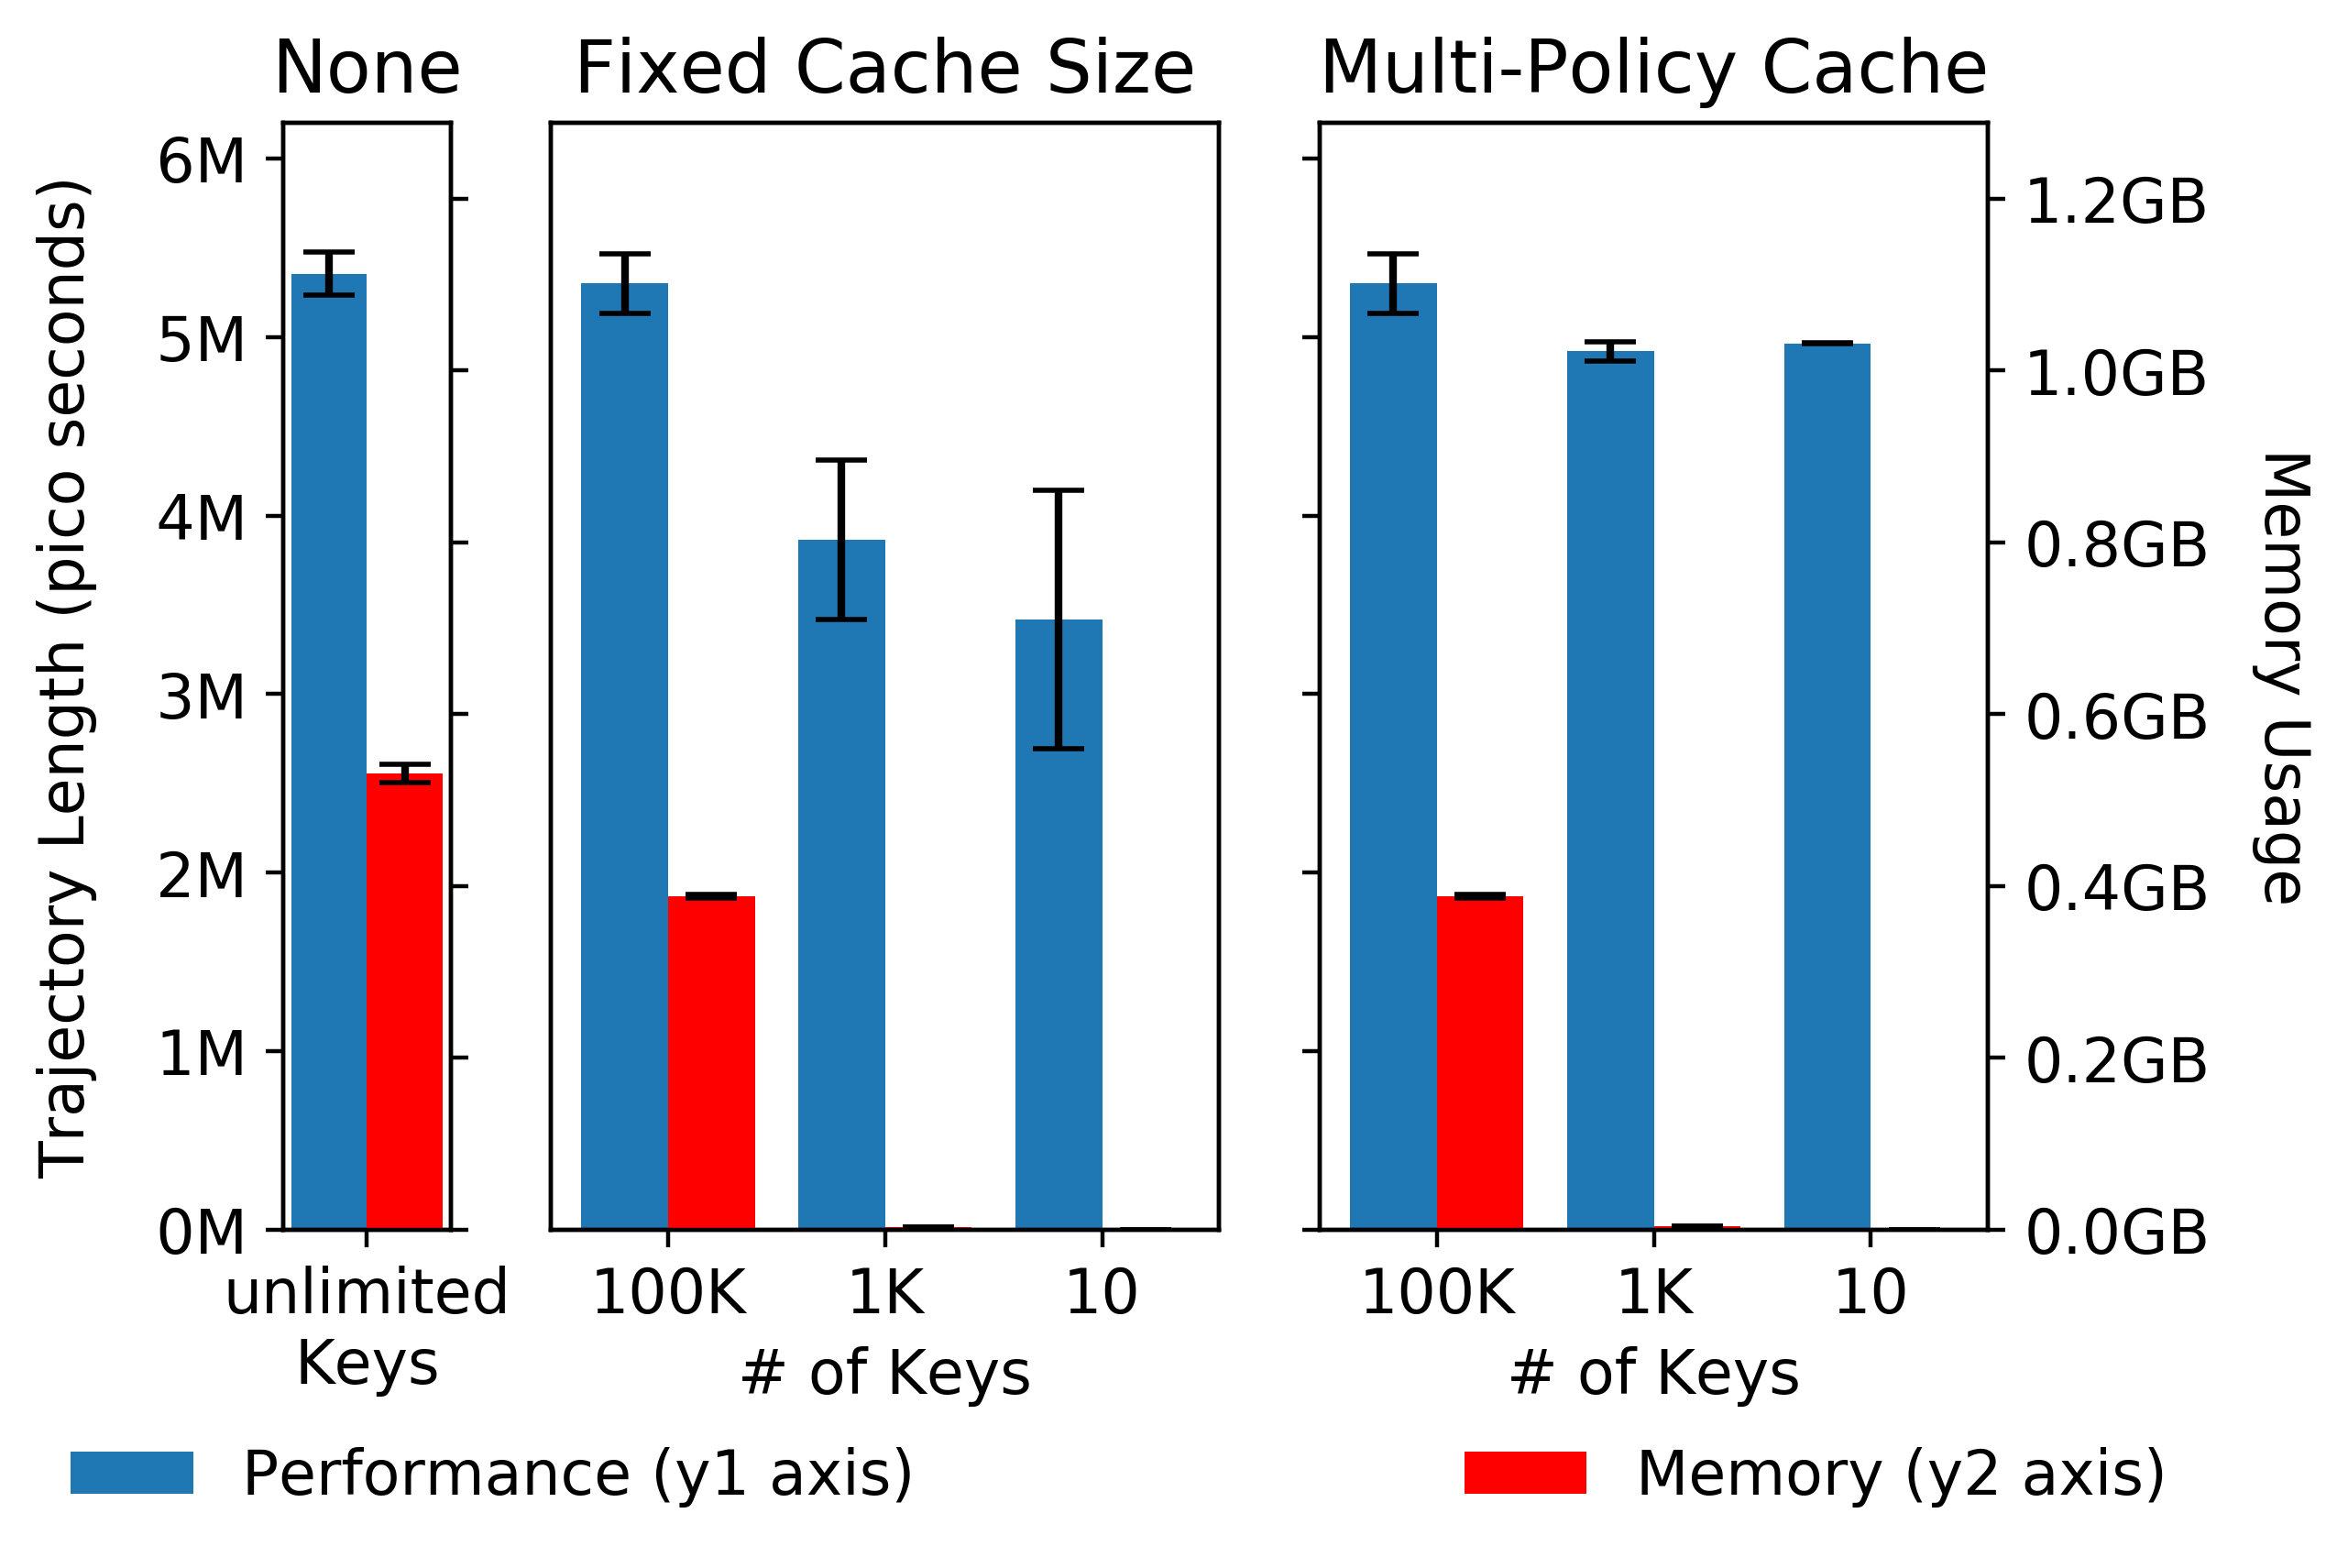
\includegraphics[width=0.5\textwidth]{figures/methodology-tradeoff.png}\\
\caption{The performance and resource utilization trade-off for different cache
management policies. ``None" is ParSplice unmodified, ``Fixed Sized Cache"
limits the size of the cache by evicting the least recently used items, and
``Multi-Policy Cache" switches to a fixed sized cache after absorbing the
initial burstiness of the workload.  The size of the fixed sized cache for each
experiment is on the \(x\) axis.  \label{fig:methodology-tradeoff}}
\end{figure}
%
%\footnotesize \centering \begin{minted}[xleftmargin=3em,linenos]{lua} function
%when() if server[whoami]['cachesize'] > n then return true end return false
%end
%
%function howmuch() if servers[whoami]['cachesize'] > n return
%servers[whoami]['cachesize'] - n end return 0 end \end{minted} \caption{Policy
%that implements a basic LRU cache. The performance and memory utilization for
%different values of \(n\) are graphed in
%Figure~\ref{fig:methodology-tradeoff}.  \label{src:lru}} \end{figure}

% why is the performance lower for smaller caches?
Although the keyspace grows to 150K, a 100K key cache achieves 99\% of the
performance. Decreasing the cache degrades performance and predictability.
Despite the memory savings, our results suggest that a multi-policy cache management strategy
could save even more memory.  The middle plot in
Figure~\ref{fig:methodology-tradeoff} show that a 100K key cache is sufficient
as a static policy but the top graph in Figure~\ref{fig:motivation-regimes}
indicates that the cache size could be much smaller. That graph shows that the
beginning of the run is characterized by many reads to a small set of keys and
the end sees much lower reads per second to a larger keyspace. Specifically, it
shows only about 100 keys as active in the latter half of the run.

After analyzing traces, we see that the 100 key cache is insufficient because
the persistent database cannot service the read-write traffic.  According to
Figure~\ref{fig:motivation-regimes}, the read requests arrive at 750 reads per
second in addition to the writes that land in each tier (about 300 puts/second,
some redundant). This traffic triggers a LevelDB compaction and reads block,
resulting in very slow progress.  Traces verify this hypothesis and show reads
getting backed up as the read/write ratio increases. To recap, small caches
incur too much load on the persistent database  at the beginning of the run but
should suffice after the initial read flash crowd passes because
the keyspace is far less active. This suggests a multi-policy cache management
strategy.

%% Why is this a good idea
%Although ParSplice does not use a distributed file system, its workload is very
%similar because the minima key-value store responds to small and frequent
%requests, which results in hot spots and flash crowds.  Modern distributed file
%systems have found efficient ways to measure, migrate, and partition metadata
%load and have shown large performance gains and
%better scalability~\cite{zheng:pdsw2014-batchfs, zheng:pdsw2015-deltafs,
%grider:pdsw2015-marfs, ren:sc2014-indexfs, patil:fast2011-giga+,
%brandt:msst2003-lh}.  Previous work quantified the speedups achieved with
%Mantle and formalized balancers that were good for file systems.

The plot on the right side of Figure~\ref{fig:methodology-tradeoff} shows the results of using Mantle
to program a multi-policy cache management strategy into ParSplice that switches between
two policies:

\begin{itemize}
  \item unlimited growth policy: cache increases on every write
  \item \(n\) key limit policy: cache constrained to \(n\) keys
\end{itemize}

The actual policy is shown and described in more detail in the next section in
Figure~\ref{src:lru-dyn}.  We trigger the policy switch at 100K keys to absorb
the flash crowd at the beginning of the run. Once triggered, keys are evicted
to bring the size of the cache down to the threshold.  In the bar chart, the
cache sizes for the \(n\) key limit policy are along the \(x\) axis.

% results: same level of performance can be achieved 
The multi-part policies show better performance than the single \(n\) key
policies. The performance and memory utilization for a 100K key cache size is
the same as the 100K bar in the ``Multi-Part Policy" graph in  Figure~\ref{fig:methodology-tradeoff} but
the rest reduce the size of the keyspace after the read flash crowd.  We see
the worst performance when the engine switches to the 10 key limit policy,
which achieves 94\% of the performance while only using 40KB of memory. 

% caveats: it is calculating 90% of the trajectory, memory value reported is final
\subsubsection*{Caveats}

The results in Figure~\ref{fig:methodology-tradeoff} are slightly deceiving for
two reasons: (1) segments take longer to generate later in the run and (2) the
memory footprint is the value at the end of 2.5 hours.  For (1), the trajectory
length vs vs.  wall-clock time curves down over time; as the nanoparticle grows
it takes longer to generate segments so by the time we reach 2 hours, over 90\%
of the trajectory is already generated.  For (2), the memory footprint is rises
until we reach 100K key switch threshold at 0.4GB, as shown by the
``\(\Delta_1\), Multi-Policy" curve in Figure~\ref{fig:memory-vs-time} but in
Figure~\ref{fig:methodology-tradeoff} we plot the final value. As a result, we
can only conclude that this policy only works well for this 2.5 hour run.

% but the result is still valid
Despite these caveats, the result is still valid: we found multi-policy cache 
management strategy that absorbs the cost of a high read throughput on a small
keyspace and reduces the memory pressure for a 2.5 hour run. Our experiments
show the effectiveness of the policy engine we integrated into
ParSplice, not that we were able to identify the best policy for all system
setups ({\it i.e.} different ParSplice parameters, number of worker tasks, and
job lengths).  To solve that problem, we need a way to identify what thresholds
we should use for different job permutations.

\section{Cache Management Using Domain-Specific Application Knowledge}
\label{sec:dom-specific}

\begin{figure*}[t!]
    \begin{subfigure}[t]{0.32\textwidth}
	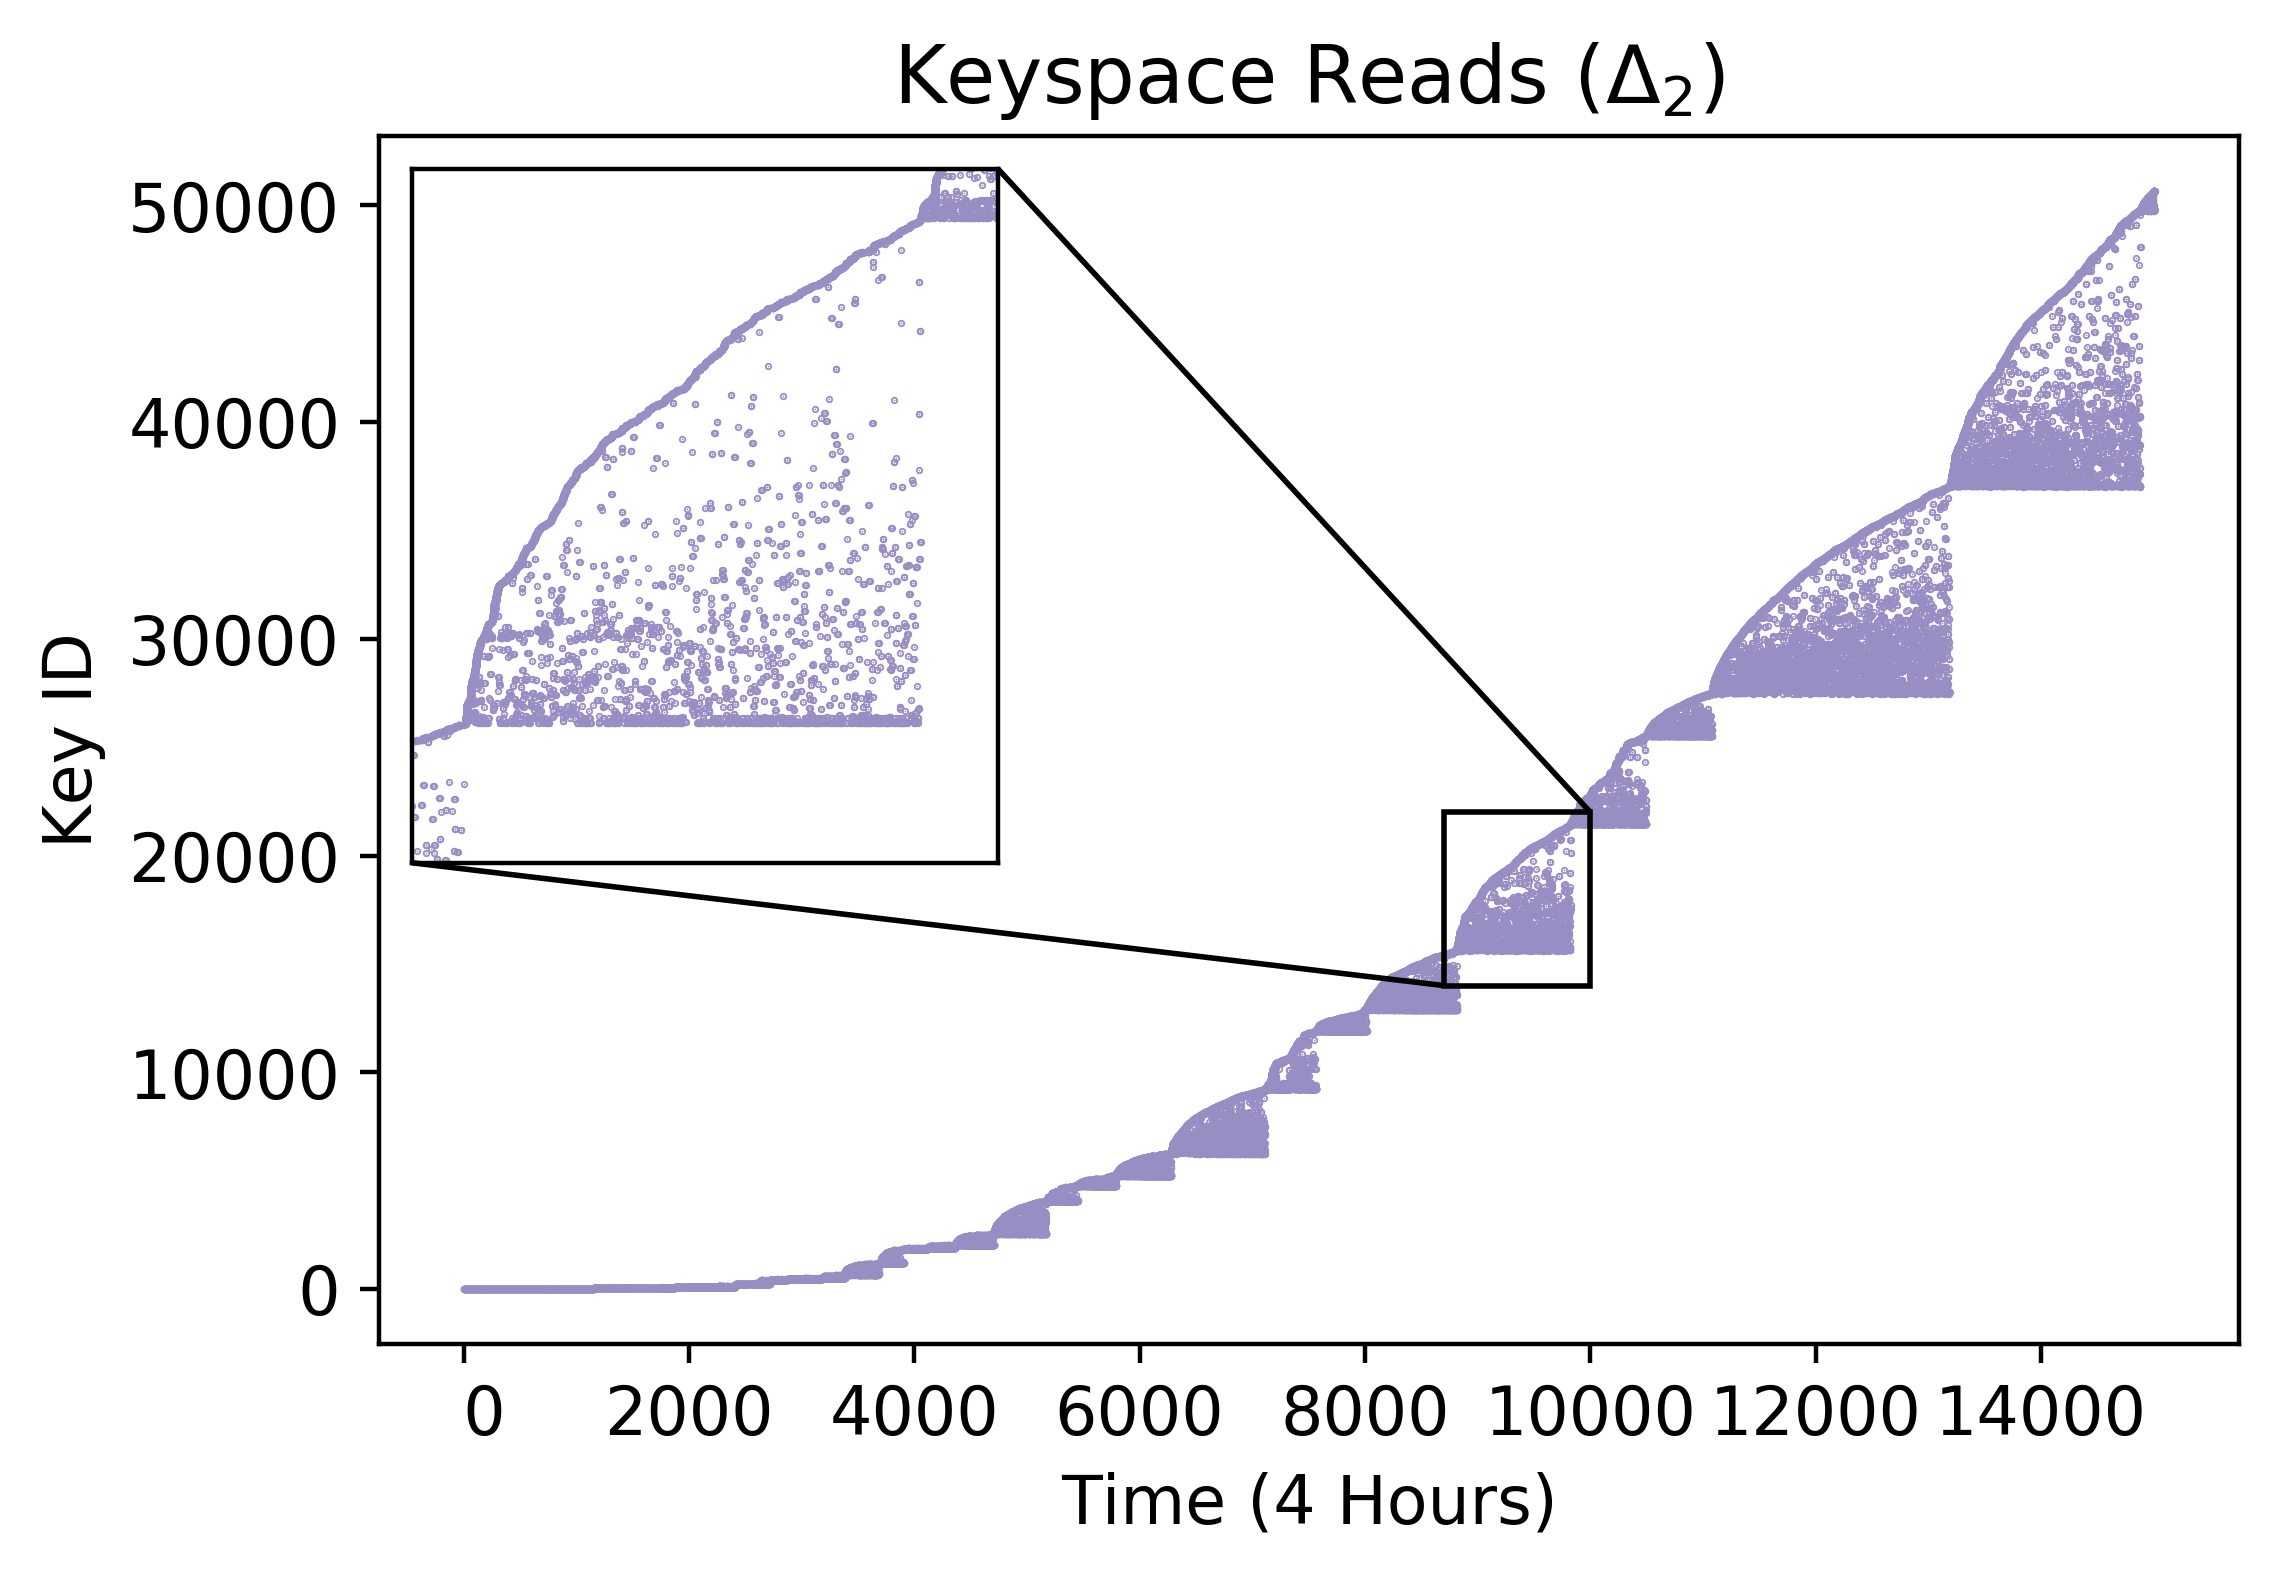
\includegraphics[width=0.9\textwidth]{figures/keyspace-zoomed.png}\\
\caption{Key activity for a 4 hour run shows groups of accesses to the same
subset of keys. Detecting these access patterns leads to a more accurate cache
management strategy, which is discussed in
Section~\S\ref{sec:regime-detection}.\label{fig:keyspace-zoomed}}
    \end{subfigure}%
    ~ 
    \begin{subfigure}[t]{0.32\textwidth}
        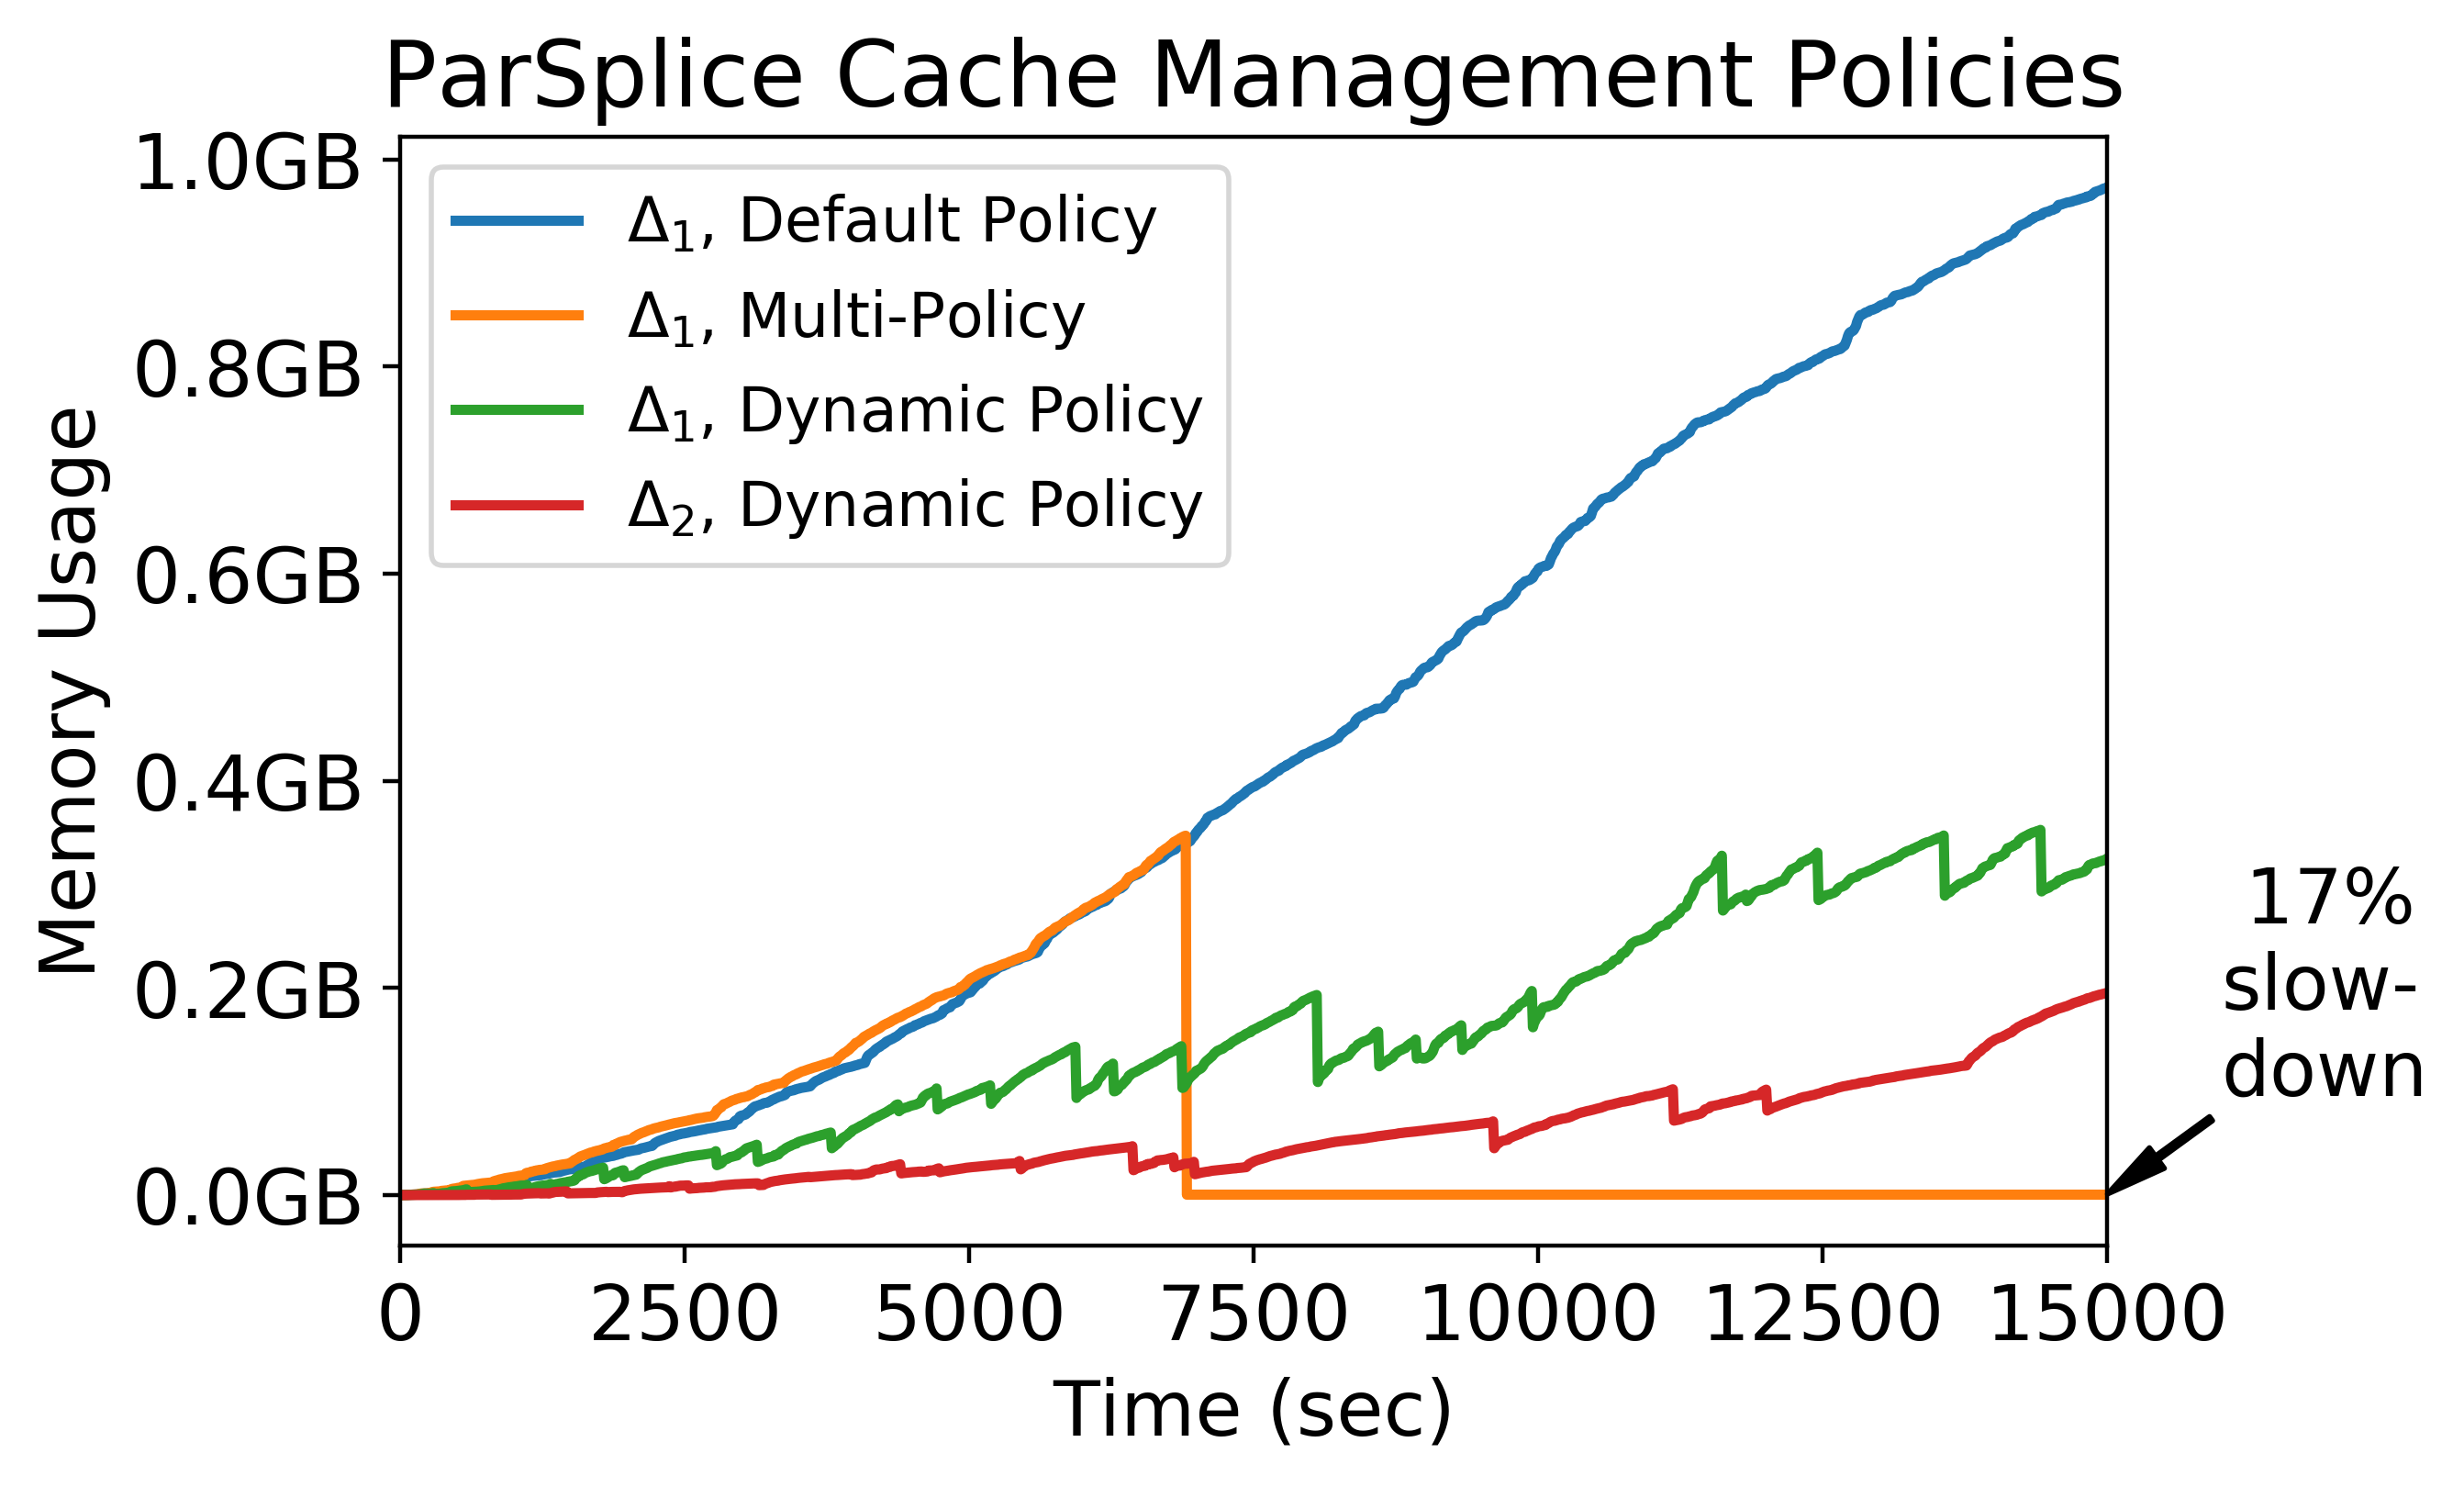
\includegraphics[width=1\textwidth]{figures/memory-vs-time.png}\\
	\caption{Memory utilization for ``No Cache Management" (unlimited cache
growth), ``Multi-Policy" (absorbs initial burstiness of workload) , and
``Dynamic Policy" (sizes cache according to key access patterns).
\label{fig:memory-vs-time}}
    \end{subfigure}%
    ~
    \begin{subfigure}[t]{0.32\textwidth}
        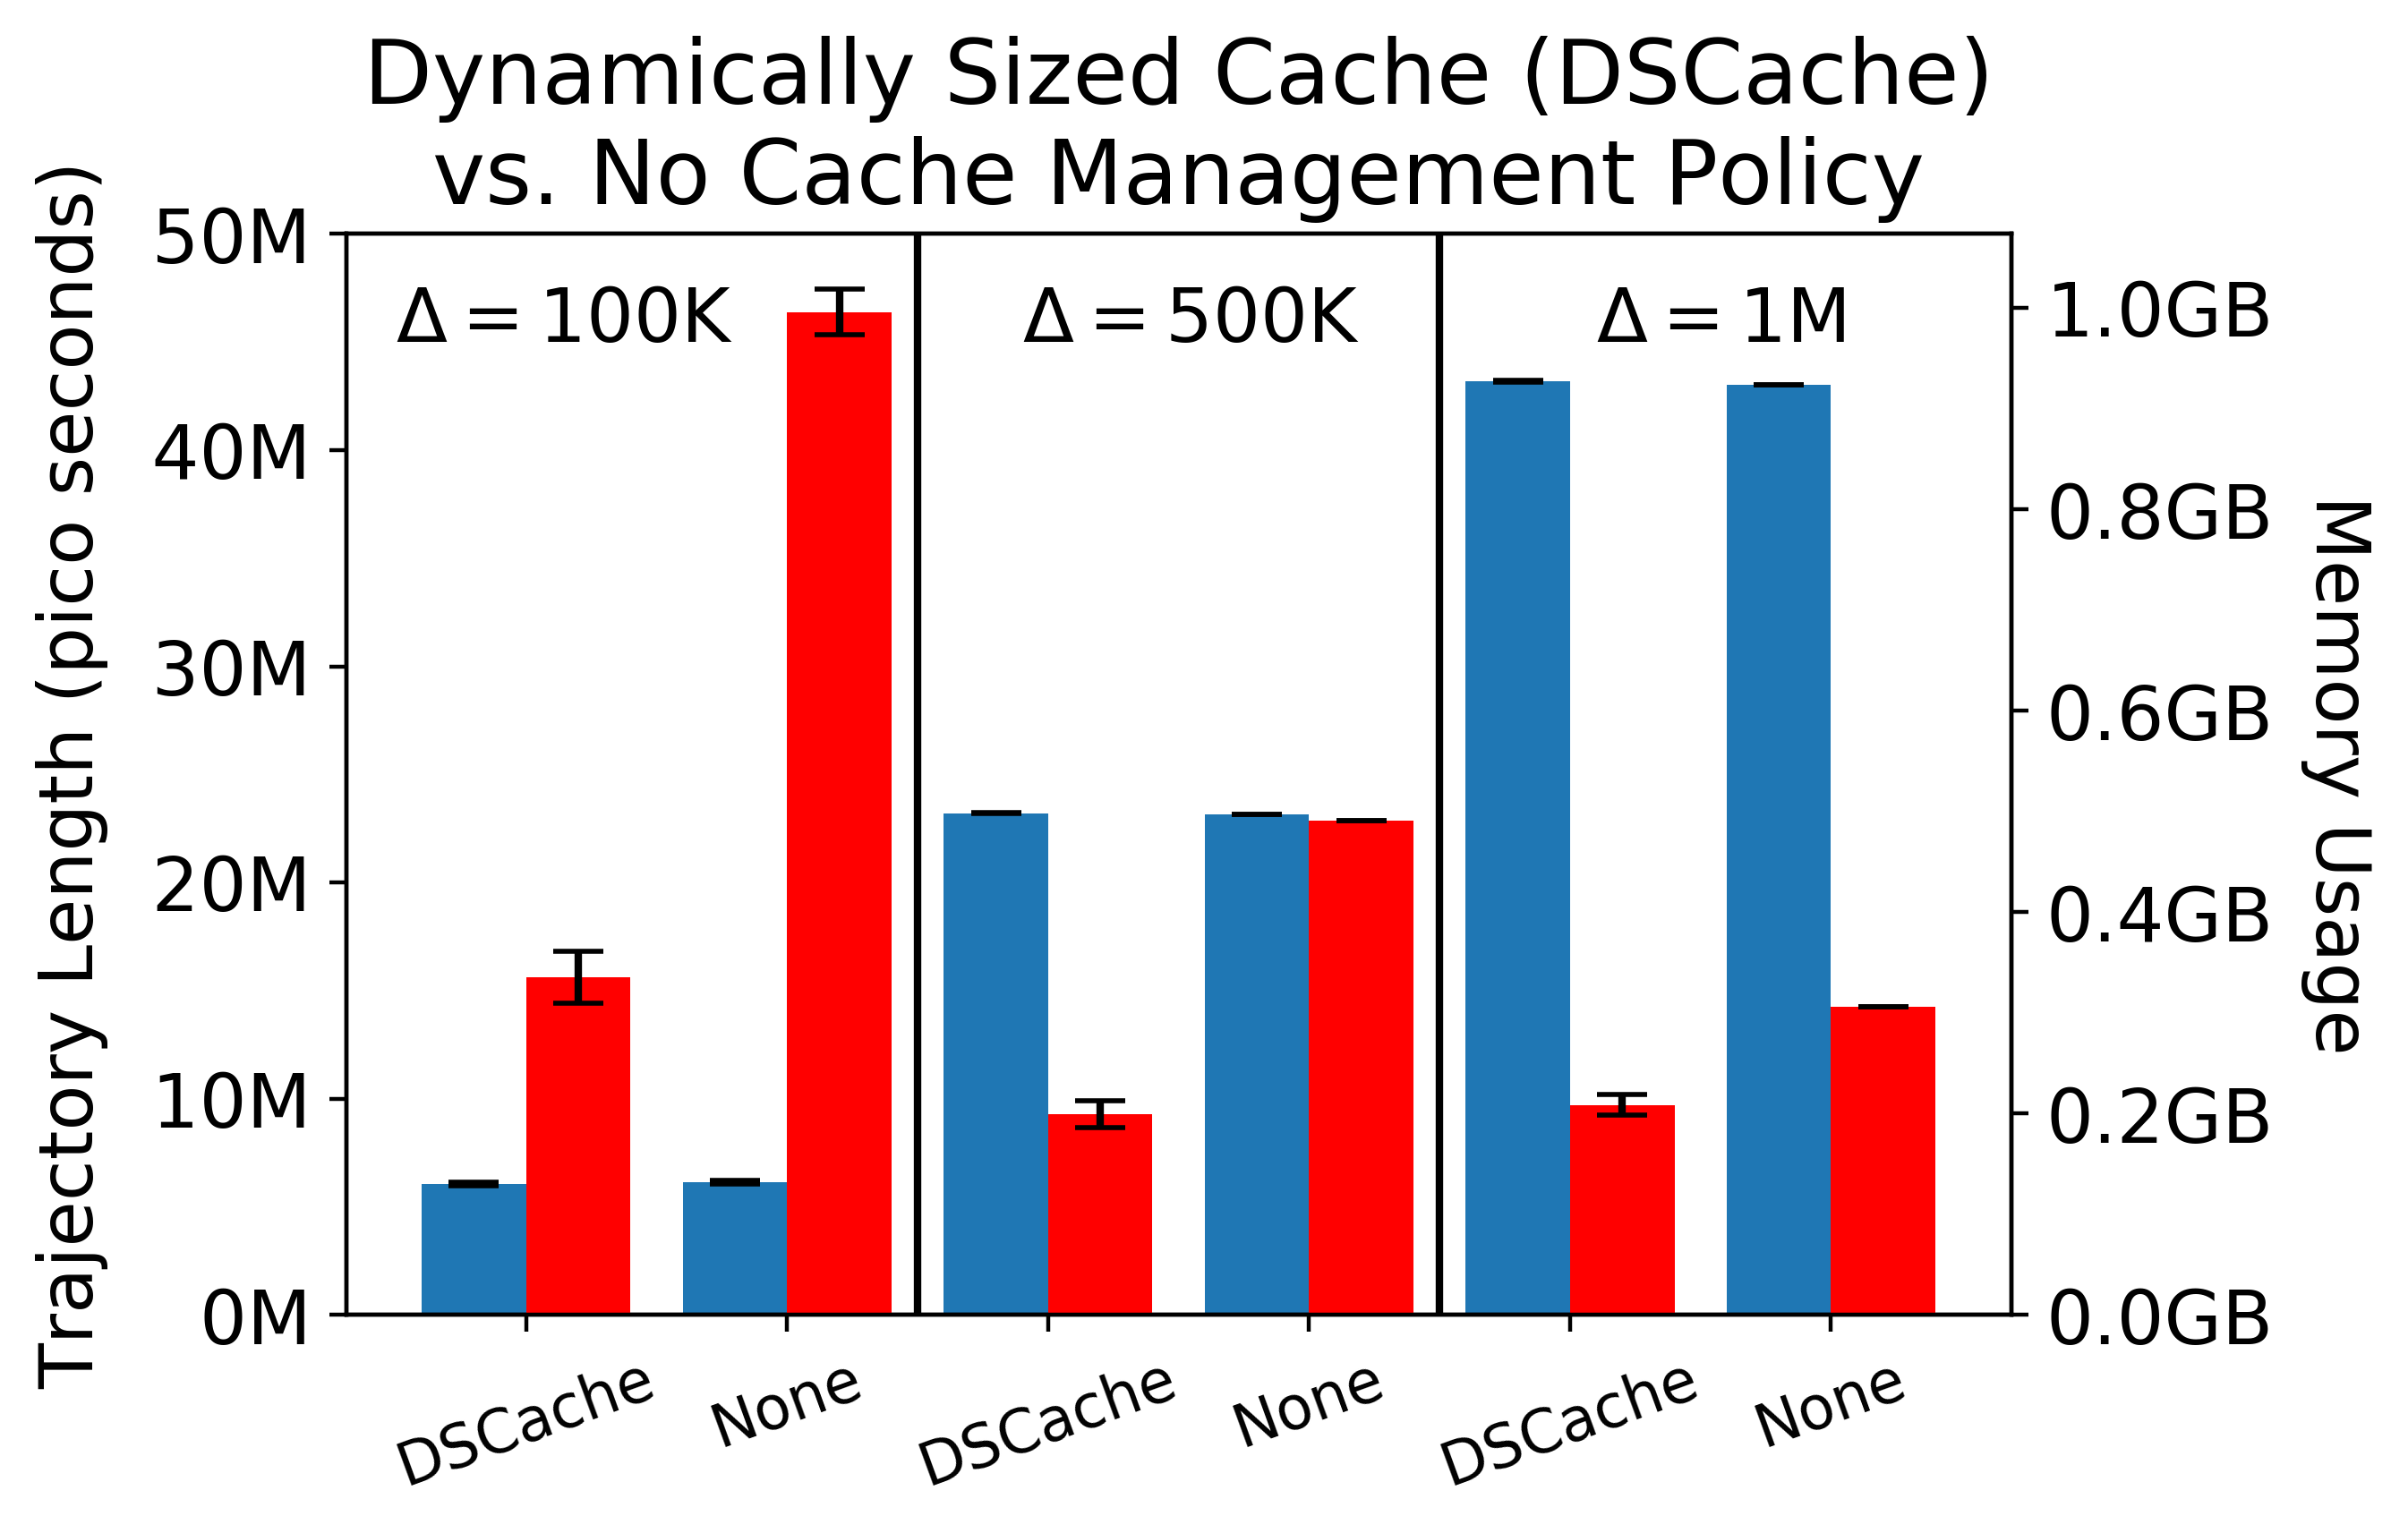
\includegraphics[width=1\textwidth]{figures/dscache-vs-none.png}\\
	\caption{Performance/Utilization for dynamically sized cache (DSCache)
policy. With negligible performance degradation, DSCache adjusts to different
\(\Delta\)s over 2\(\times\) memory in the best case.
\label{fig:dscache-vs-none}}
    \end{subfigure}%
    \caption{Different cache management policies tested over the Mantle policy engine.}
\end{figure*}

%\begin{figure}[t]
%  \noindent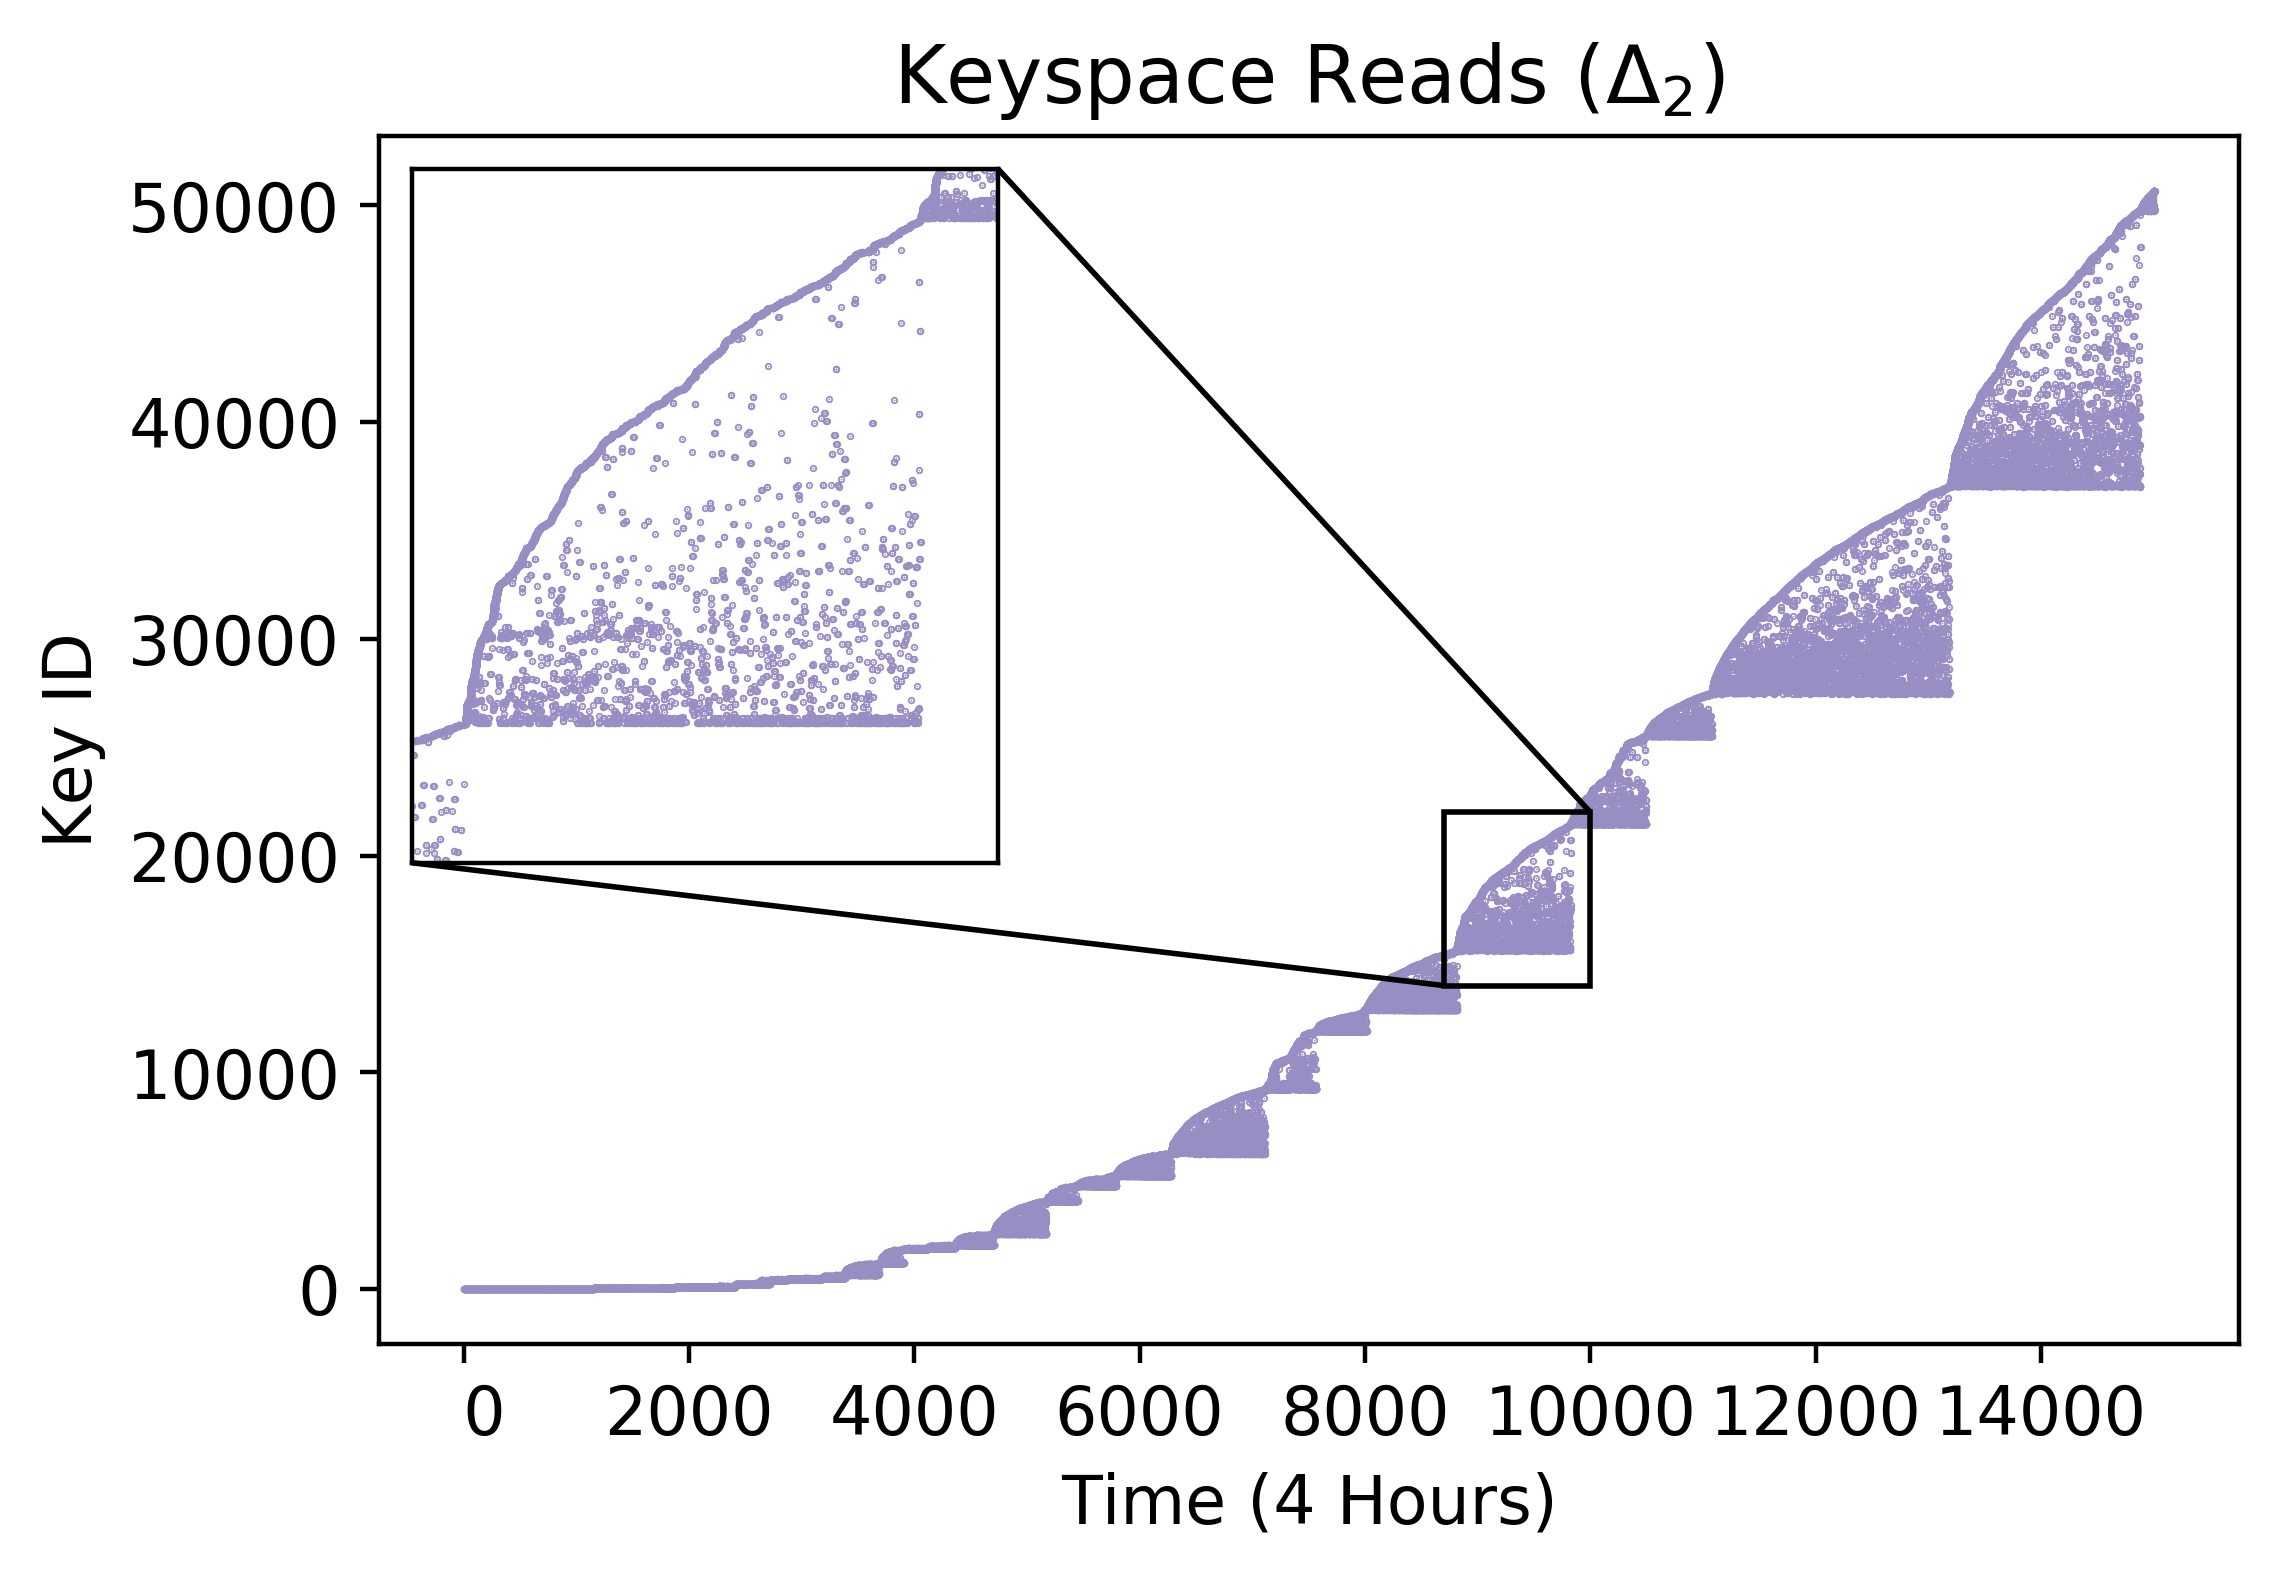
\includegraphics[height=5cm,width=0.4\textwidth]{figures/keyspace-zoomed.png}\\
%
%  \caption{Key activity for a 4 hour run shows groups of accesses to the same
%  subset of keys. Detecting these access patterns leads to a more accurate cache
%  management strategy.\label{fig:keyspace-zoomed}}
%
%\end{figure}
%
%\begin{figure}[t]
%\noindent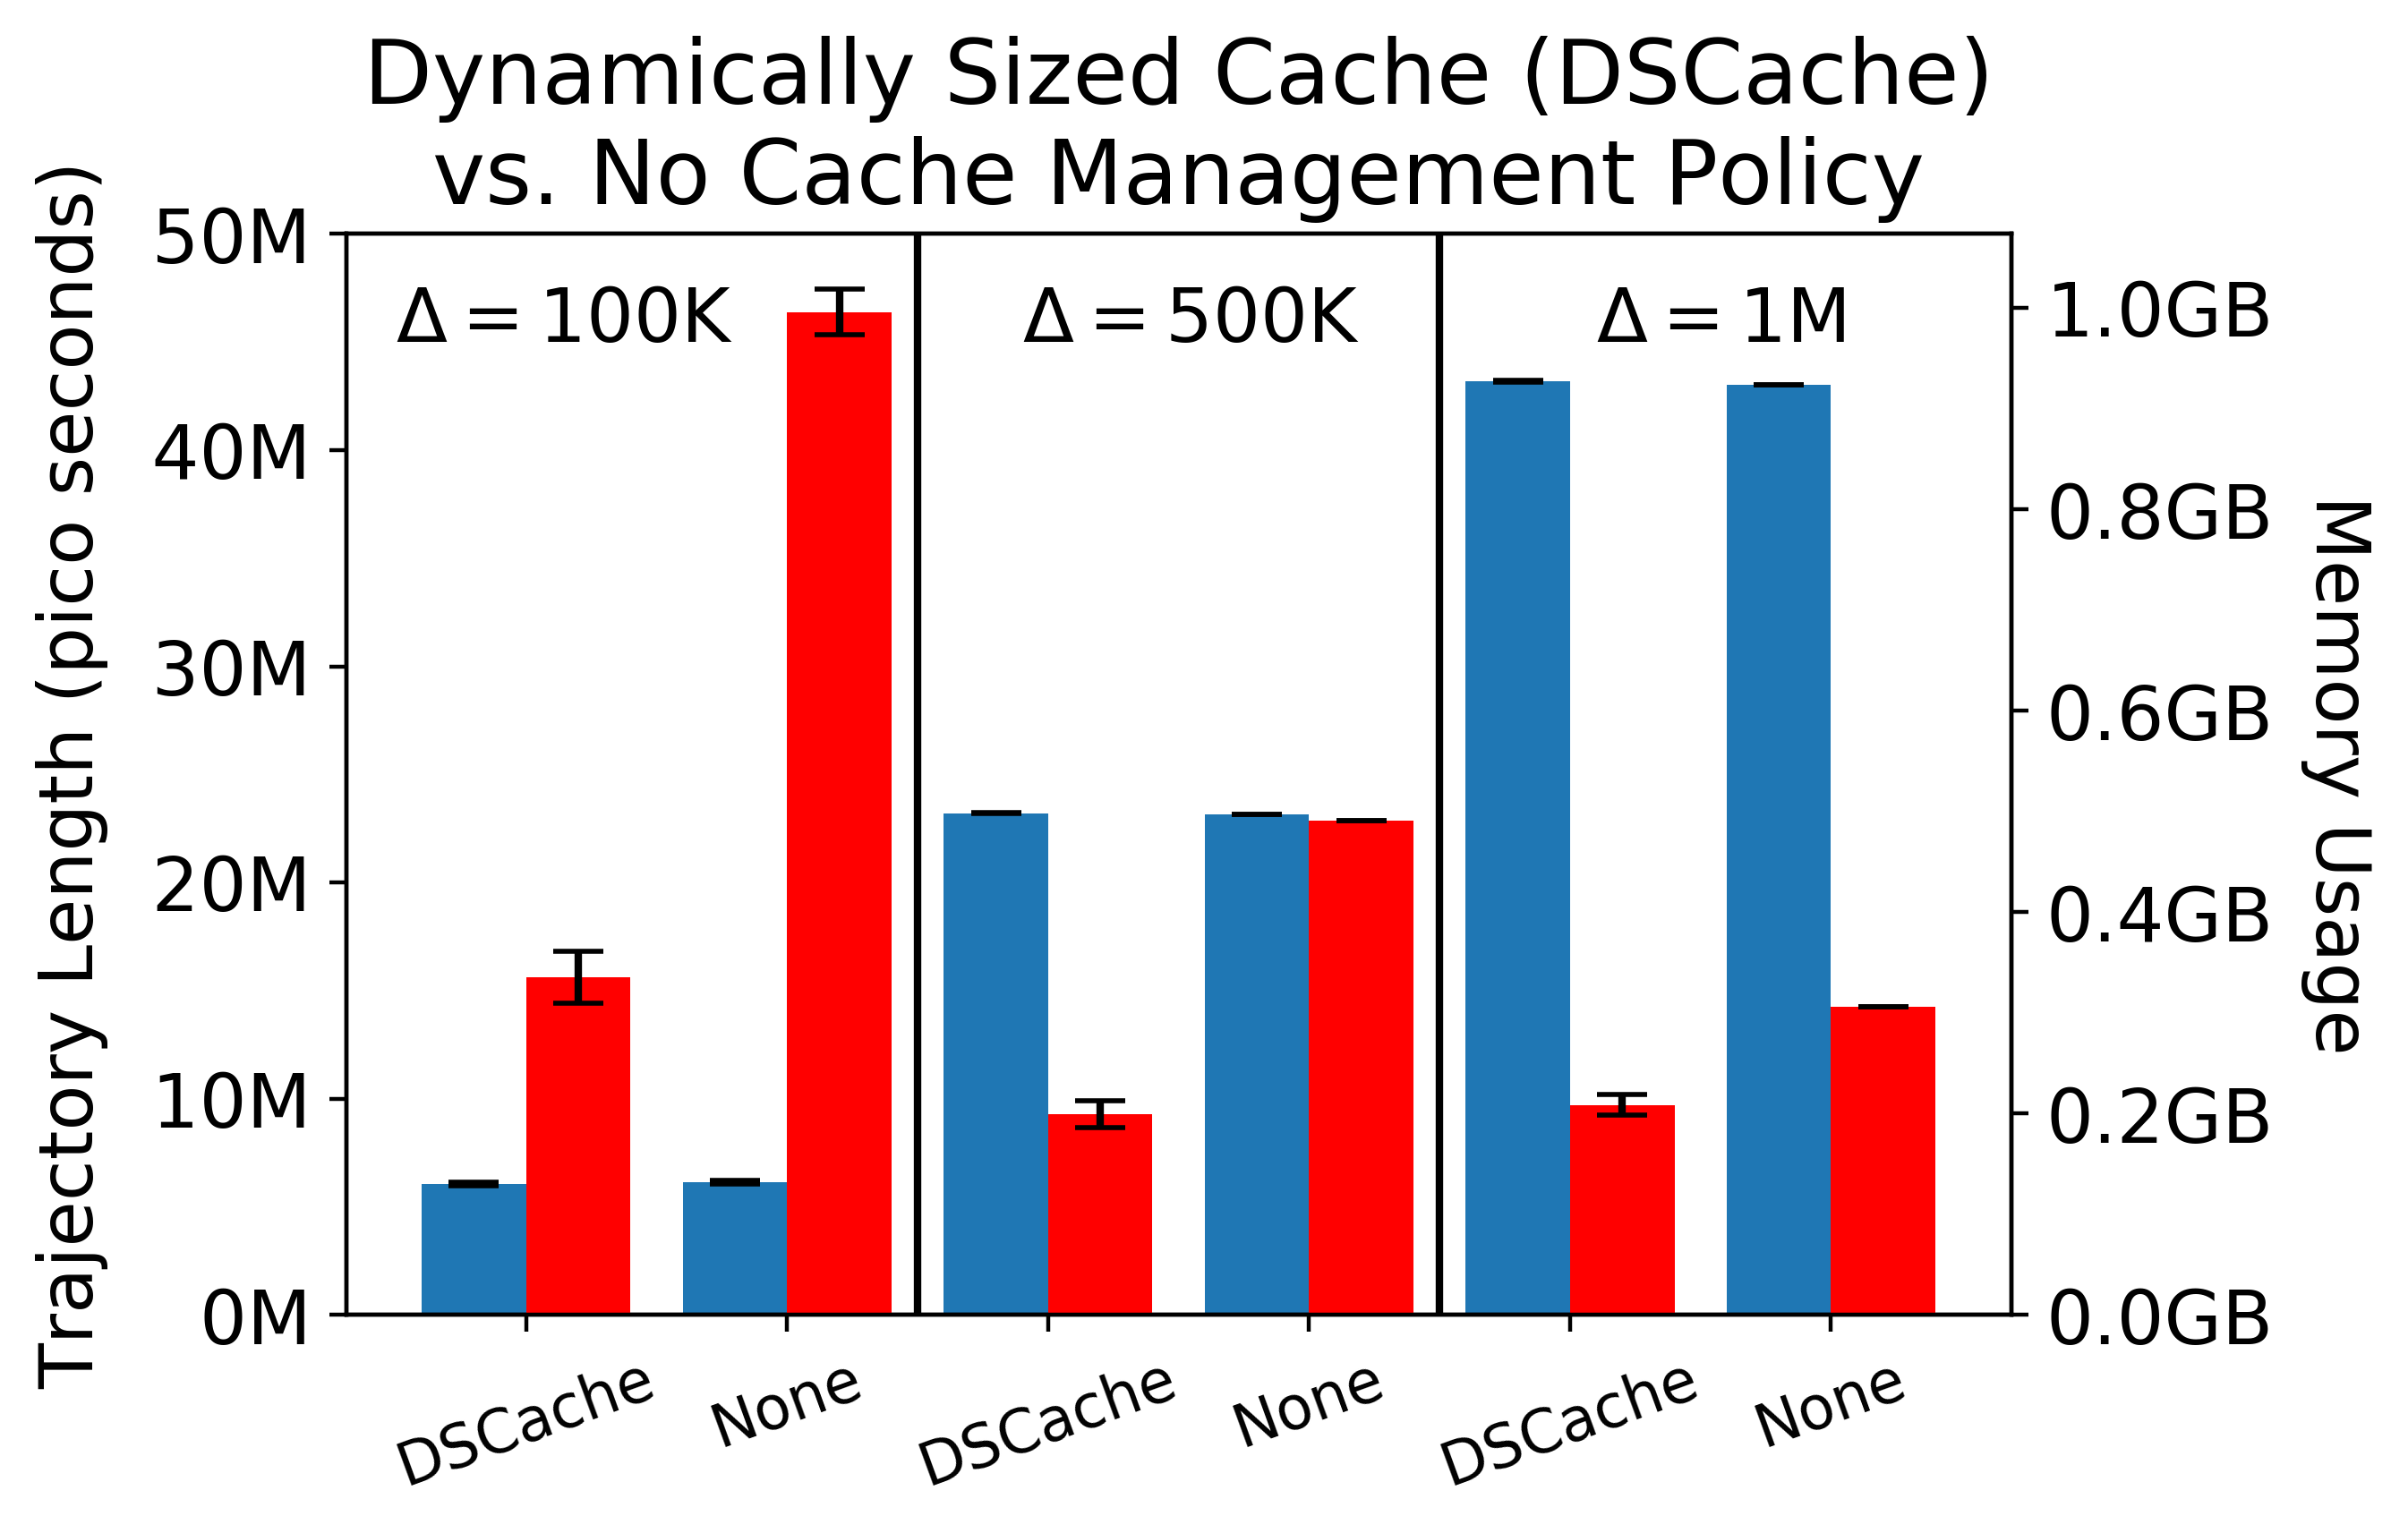
\includegraphics[width=0.5\textwidth]{figures/dscache-vs-none.png}\\
%
%\caption{The performance and resource utilization trade-off for the dynamically
%sized cache (DSCache) policy compared to no cache management. With a negligible
%performance impact, DSCache adjusts to different initial conditions
%(\(\Delta\)) automatically and saves over 2\(\times\) memory in the best case.
%\label{fig:dscache-vs-none}}
%\end{figure}
%
%\begin{figure}[t]
%\noindent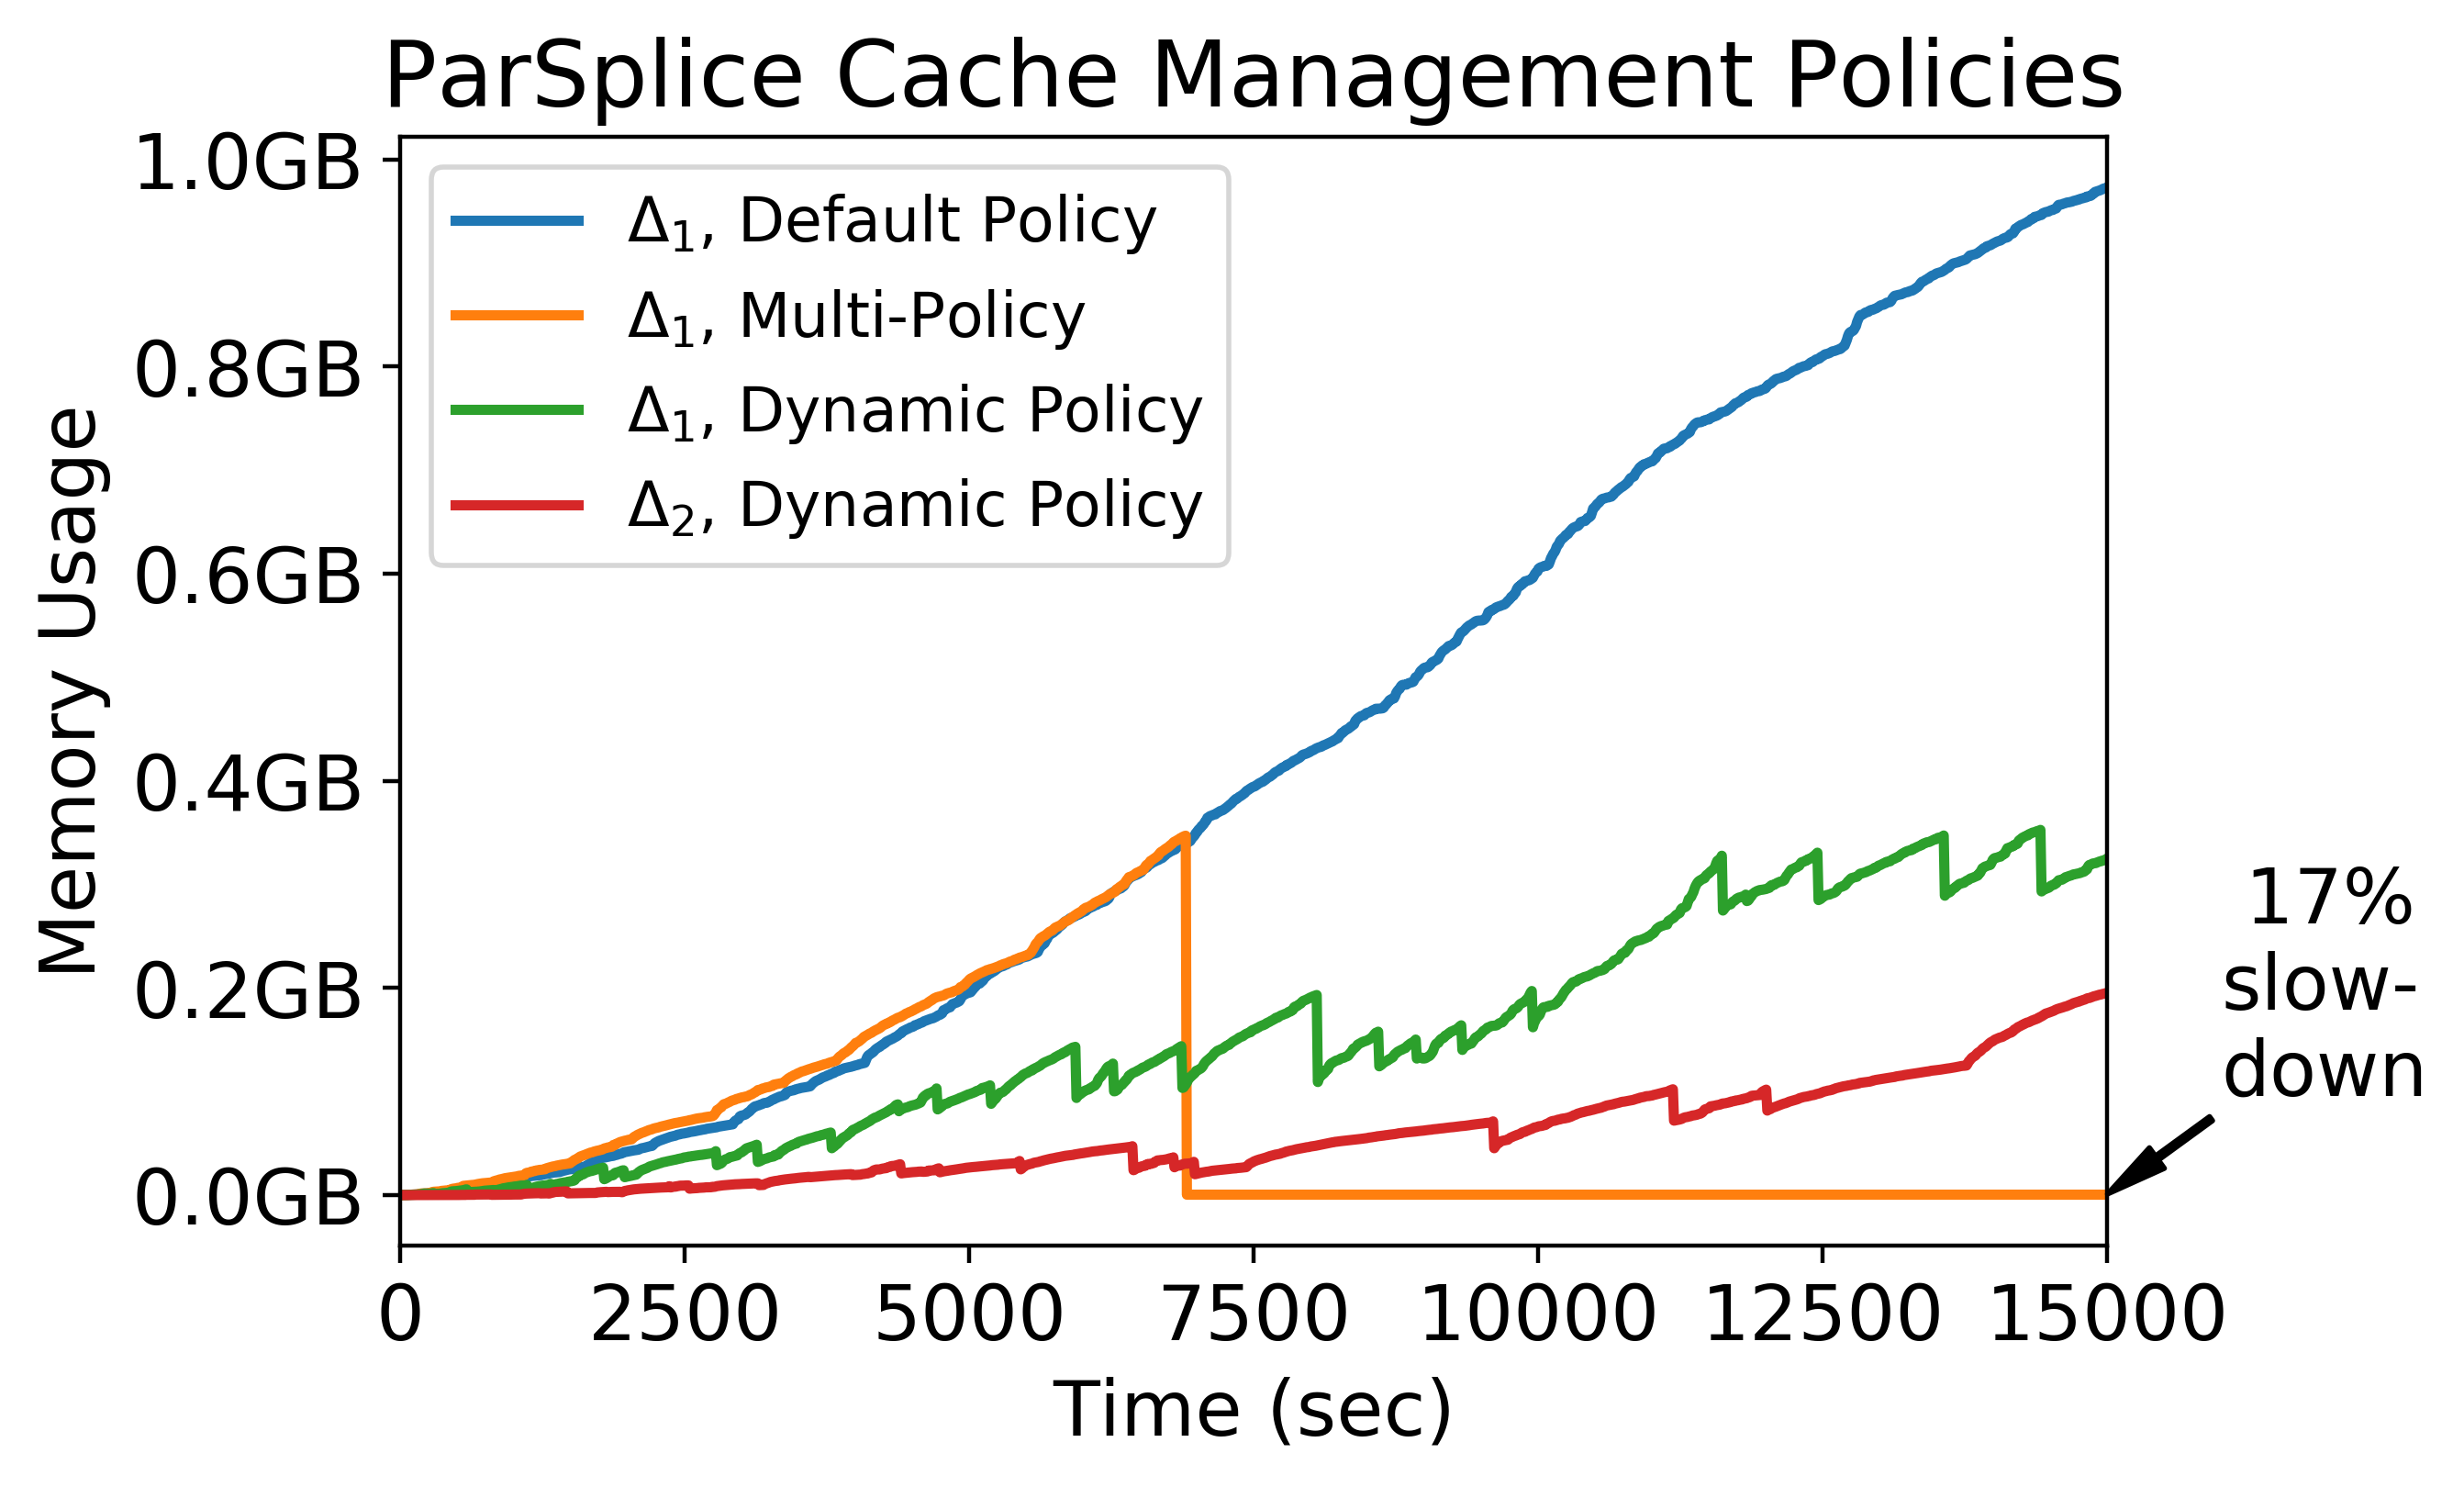
\includegraphics[width=0.5\textwidth]{figures/memory-vs-time.png}\\
%
%\caption{Memory utilization of different cache management policies.  ``No Cache
%Management" allows unlimited cache growth, ``Multi-Policy" absorbs the initial
%burstiness of the workload before switching to a more constrained cache, and
%the ``Dynamic Policy" curves size the cache according to key access patterns.
%We show a \(\Delta_2\) growth rate to demonstrate the dynamic policy's ability
%to adjust to a different set of initial conditions.\label{fig:memory-vs-time}}
%\end{figure}

Feeding domain-specific knowledge about the ParSplice application into a policy
leads to more a accurate cache management strategy.
Figure~\ref{fig:keyspace-zoomed} shows which keys (\(y\) axis) are accessed by
the ParSplice tasks over time (\(x\) axis). The groups of accesses to a subset
of keys, which we call an access ``fan" in subsequent sections, occurs because
molecules are stuck in deep trajectories. Recall that the in-memory database
stores the molecules' EOM minima, which is the smallest effective energy that a
molecule observes during its trajectory. So molecules stuck in deep
trajectories explore the same minima until they can escape to a new set of
states. This exploration of the same set of states is called a superbasin. 

Detecting these superbasins can lead to more effective cache management
strategies because the height of the groups of key accesses is ``how much" of cache
to evict and the width of the groups of key accesses is ``when" to evict values from
the cache.  The zoomed portion of Figure~\ref{fig:keyspace-zoomed} shows how a
single superbasin affects the key accesses. Moving along the \(x\) axis shows
that the number of unique keys accessed over time grows while moving along the
\(y\) axis shows that early keys are accessed more often.  Overall, superbasins
are never re-visited because the simulation only adds molecules; we can never
reach a state with less molecules. This is why keys are never re-accessed.
Despite these patterns, the following characteristics of superbasins make it
hard to detect them:

\begin{itemize}

  \item superbasin key accesses are random and there is no threshold ``minimum distance
  between key access" that indicates we have moved on to a new superbasin

  \item superbasins change immediately

  \item the number of keys a superbasin accesses differs from other superbasins

\end{itemize}

Below we describe the policies we implemented and deployed using Mantle.

\subsection{Failed Strategies}

To detect the access patterns in Figure~\ref{fig:keyspace-zoomed}, we try a
variety of techniques using Mantle. Unfortunately, we found that they all
proliferated more parameters that need to be tuned. Furthermore, we find that
many of the metrics do not signal a new fans, that our metrics are not accurate
enough, and that even if we tune all parameters they still will not work for
all initial conditions.  Below, we indicate which parameters we need to add for
each technique and the value we find to work best, via tuning and parameter
sweeps, for one set of initial conditions.

\begin{itemize}

  \item Statistics: decay on each key counts down until 0 0-valued keys are
evicted.  ``history-of-key-accesses", set to 10 seconds, to evict keys.

  \item Calculus: use derivative to strip away magnitudes; use large positive
slopes followed large negative slope as signal for new fan. ``Zero-crossing"
for distance between small/large spikes to avoid false positives, set to 40
seconds; `window size", set to 200 seconds, for the size of the moving average 

  \item K-Means Clustering fails because ``K" is not known {\it a-priori} and
fans are different size. ``K", set to 4, for the number of clusters in the data
using the sum of the distances to the centroid

  \item DBScan: finds clusters using density as a metric. ``Eps", set to 20, for
max distance between 2 samples in same neighborhood; ``Min", set to 5, for the
number of samples per core

  \item Anomaly Detection: size of the image is too big and bottom edges are
not thick enough

\end{itemize}

\subsection{Dynamically Sized Cache: Access Pattern Detection}
\label{sec:regime-detection}

Figure~\ref{src:dyn-cache} shows the algorithm we use to detect the key access
patterns. Iterating backwards through the key access trace, at each time step we
find the lowest key ID and compare against the lowest key ID we have seen so
far (Line 7). We also maintain the top and bottom of each fan (Line 13) so we
can tell the ``how much" policy the number of keys to evict (Line 19).  The
algorithm iterates backwards over the key access trace because a change in the
minimum value signals a new fan. No signal exists iterating left to right, as
the maximum value always increases and the minimum values at the bottom of each
fan are sparse.  For example, the maximum distance between values along the
bottom edge of the zoomed fan in Figure~\ref{fig:keyspace-zoomed} is 125
seconds, while the maximum distance between minimum values for the fan before
is 0 seconds. As a result of this sparseness, iterating left to right requires
a ``window size" parameter to determine when we think a minimum value will not
show up again.  We exchange runtime, in the form of an O(\(n\)) algorithm where
\(n\) is the number events, for simplicity because this approach avoids adding
new thresholds for fan detection ({\it e.g.}, space between key accesses, space
between key IDs, and window size of consecutive key accesses).

The performance and memory utilization is shown by the ``DSCache" bars in
Figure~\ref{fig:dscache-vs-none}. Without sacrificing performance (trajectory
length), the dynamically sized cache policy uses between 32\%-66\% less memory
than the default ParSplice configuration (no cache management) for the 3
initial conditions we test. The memory usage is shown by the ``Dynamic Policy"
curves in Figure~\ref{fig:memory-vs-time}, where the behavior mirrors the key
access patterns in Figure~\ref{fig:keyspace-zoomed}. We also show a
\(\Delta_2\) growth rate to demonstrate the dynamic policy's ability to adjust
to a different set of initial conditions.

%For points \(z\), \(y\), and \(x\), if the
%local minimum is the same we are in a regime.  Processing \(y\), we set the
%local minimum to be \(min(y, m_l)\), where \(m_l\) is the local minimum of the
%previous time step of \(z\).  The algorithm incorrectly detects a regime change
%if the local minimum of \(y\) is lower than local minimum of \(z\), since \(y\)
%may have points {\it within} \(z\); recall that we are trying to detect the
%whole fan, not just the bottom edge of each fan. 

\begin{figure}[h]
\footnotesize
\begin{minted}[xleftmargin=3em,linenos]{lua}
d = timeseries()          -- provided by mantle
ts, id = d:get(d:size())  -- provided by mantle
fan  = {start=nil, finish=ts, top=0, bottom=id}
fans = {}
for i=d:size(),1,-1 do    -- detect all fans
  ts, id = d:get(i)
  if id < fan['bottom'] then
    fan['start']  = ts
    fans[#fans+1] = fan 
    fan = {start=nil, finish=ts, top=0, bottom=id}
  end 

  if id > fan['top'] then fan['top'] = id end 
end
fan['start'] = 0 
fans[#fans+1] = fan 

if #fans < 2 then return false else
  WRstate(fans[#fans-1]['top']-fans[1]['bottom'])
  return true
end
\end{minted}
\caption{The dynamically sized cache policy, whose performance is shown in 
Figure~\ref{fig:cache-management}, iterates backwards over timestamp-keyID pairs
and detects when key accesses move on to a new subset of
keys.\label{src:dyn-cache}}
\end{figure}
